\newpage\setcounter{dang}{0}
\section{VECTƠ TRONG MẶT PHẲNG TỌA ĐỘ}
\subsection{Tóm tắt lí thuyết}
\begin{tomtat}
\subsubsection{TRỤC VÀ ĐỘ DÀI ĐẠI SỐ TRÊN TRỤC}
\begin{enumerate}
\item \textbf{Trục tọa độ}
	\begin{dn} 	
	\end{dn}
	\begin{itemize}
		\item Trục tọa độ (hay gọi tắt là trục) là một đường thẳng trên đó đã xác định một điểm $O$ gọi là điểm gốc và một vectơ đơn vị $\overrightarrow{e}$.
		\item Điểm $O$ gọi là gốc tọa độ.
		\item Hướng của vectơ đơn vị là hướng của trục.
		\item Ta kí hiệu trục đó là $(O;\overrightarrow{e})$. 
	\end{itemize}
	\begin{center}
		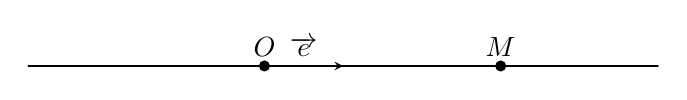
\begin{tikzpicture}[line cap=round,line join=round,>=stealth,x=1.0cm,y=1.0cm,scale=1]
		\draw (-3,0)--(5,0);
		\draw [->] (0,0) node [above] {$ O $}--(1,0);
		\draw (0.5,0) node[above] {$ \overrightarrow{e} $};		
		\fill[black](0,0) circle (2pt) (3,0) node[above] {$ M $} circle (2pt);		
		\end{tikzpicture} 
	\end{center}
\item \textbf{Tọa độ của một điểm}\\
Cho $M$ là một điểm tùy ý trên trục $\left(O;\overrightarrow{e}\right)$. Khi đó có duy nhất một số $k$ sao cho $\overrightarrow{OM}=k\cdot\overrightarrow{e}$.\\
Ta gọi số $k$ đó là tọa độ của điểm $M$ đối với trục đã cho.
\item \textbf{Tọa độ vectơ}\\
	Cho hai điểm $A$ và $B$ trên trục $\left(O;\overrightarrow{e}\right)$.\\
	Khi đó có duy nhất số $a$ sao cho $\overrightarrow{AB}=a \cdot \overrightarrow{e}$. Ta gọi số $a$ là độ dài đại số của vectơ $\overrightarrow{AB}$ đối với trục đã cho và kí hiệu $a=\overline{AB}$.\\
	\begin{nx}		
	\end{nx}
	\begin{itemize}
		\item Nếu $\overrightarrow{AB}$ cùng hướng với $\overrightarrow{e}$ thì $\overline{AB}=AB$, còn nếu $\overrightarrow{AB}$ ngược hướng với $\overrightarrow{e}$ thì $\overline{AB}=-AB$.
		\item  Nếu hai điểm $A$ và $B$ trên trục $\left(O;\overrightarrow{e}\right)$ có tọa độ lần lượt là $a$ và $b$ thì $\overline{AB}=b-a$.
	\end{itemize}
\end{enumerate}
\subsubsection{HỆ TRỤC TỌA ĐỘ}
\begin{enumerate}
\item \textbf{Hệ trục tọa độ}
	\begin{dn}	
			Hệ trục toạ độ $\left(O;\overrightarrow{i},\overrightarrow{j}\right)$ gồm hai trục $\left(O;\overrightarrow{i}\right)$ và $\left(O;\overrightarrow{j}\right)$ vuông góc với nhau.
	\begin{itemize}
		\item 	Điểm gốc $O$ chung của hai trục gọi là gốc tọa độ.
		\item  Trục $\left(O;\overrightarrow{i}\right)$ được gọi là trục hoành và kí hiệu là $Ox$, trục $\left(O;\overrightarrow{j}\right)$ được gọi là trục tung và kí hiệu là $Oy$. 
		\item Các vectơ $\overrightarrow{i}$ và $\overrightarrow{j}$ là các vectơ 	đơn vị trên $Ox$ và $Oy$ và $\left|\overrightarrow{i}\right|=\left|\overrightarrow{j}\right|=1$. 
		\item Hệ trục tọa độ  $\left(O;\overrightarrow{i},\overrightarrow{j}\right)$ còn được kí hiệu là $Oxy$.		
	\begin{center}
	\begin{tikzpicture}[line cap=round,line join=round,>=stealth,x=1.0cm,y=1.0cm,scale=1]
	\draw (0,0)--(5,0) (2,-2)--(2,2);
	\draw[->](2,0)--(3,0);
	\draw[->] (2,0)--(2,1);				
	\draw [->](7,0)--(13,0);
	\draw [->](9,-2)--(9,2);				
	\draw(2,0) node [below left] {$ O $} (2,0.5) node [left] {$ \overrightarrow{j} $} (2.5,0) node [below] {$ \overrightarrow{i} $};
	\draw (9,0) node [below left] {$ O $} (9,1) node [left] {$ 1 $} (10,0) node [below] {$ 1 $};
	\def\gocvuong(#1,#2,#3,#4){\coordinate (#1#2) at ($(#2)!#4 mm!(#1)$);\coordinate (#2#3) at ($(#2)!#4 mm!(#3)$);\coordinate (#1#3) at ($(#1#2)+(#2#3)-(#2)$);\draw (#1#2)--(#1#3)--(#2#3);	}
	\path 
	(9,0) coordinate (A)
	(9,1) coordinate (B)
	(10,0) coordinate (C)
				;
	\gocvuong(B,A,C,2);
	\fill (10,0) circle (1pt) (9,1) circle (1pt);
	\draw (9,2) node [right] {$ y $} (13,0) node [above] {$ x $};
	\draw (2,0) rectangle (2.2,0.2);
	\end{tikzpicture} 
	\end{center}
	\item  Mặt phẳng mà trên đó đã cho một hệ trục tọa độ $Oxy$ còn được gọi là mặt phẳng tọa độ $Oxy$.	Hay gọi tắt là mặt phẳng $Oxy$.
			\end{itemize}
	\end{dn} 
\item \textbf{Tọa độ vectơ}
	\immini{Trong mặt phẳng $Oxy$ cho một vectơ $\overrightarrow{u}$ tùy ý. Vẽ $\overrightarrow{OA}=\overrightarrow{u}$ và gọi $A_1, A_2$ lần lượt là hình chiếu vuông góc của $A$ lên $Ox$ và $Oy$. \\
	Ta có $\overrightarrow{OA}=\overrightarrow{OA}_1+\overrightarrow{OA}_2$ và cặp số duy nhất $(x;y)$ để $\overrightarrow{OA}_1=x\cdot\overrightarrow{i}$, $\overrightarrow{OA}_2=y\cdot\overrightarrow{j}$.\\
	 Như vậy $\overrightarrow{u}=x\cdot\overrightarrow{i}+y\cdot\overrightarrow{j}$.\\
	Cặp số $(x;y)$ duy nhất đó được gọi là tọa độ của vectơ $\overrightarrow{u}$ đối với hệ tọa độ $Oxy$ và viết
$\overrightarrow{u}=(x;y)$ hoặc $\overrightarrow{u}(x;y)$. Số thứ nhất $x$ gọi là hoành độ, số thứ hai $y$ gọi là tung độ của vectơ $\overrightarrow{u}$.  $$\overrightarrow{u}=(x;y)\Leftrightarrow\overrightarrow{u}=x\overrightarrow{i}+y\overrightarrow{j}.$$
	}{
	\begin{tikzpicture}[line cap=round,line join=round,>=stealth,x=1.0cm,y=1.0cm,scale=.7]
	\draw(0,-2)--(0,5) (-2,0)--(5,0);
	\draw[->] (0,0)--(0,1);
	\draw[->] (0,0)--(1,0);
	\draw[->] (0,0) -- (3,2);
	\draw[->] (1,3) -- (4,5);
	\draw (0,0) node [below left] {$ O $} (0,2) node [left] {$ A_2 $} (3,0) node [below] {$ A_1 $} (3,2) node [above right] {$ A $};
	\draw(0,0.5) node [left] {$ \overrightarrow{j} $};
	\draw (0.5,0) node[below] {$ \overrightarrow{i} $};
	\draw (1.5,1) node [below] {$ \overrightarrow{u} $};
	\draw (2.5,4) node [below] {$\overrightarrow{u}$};
	:\fill (0,2) circle (2pt) (3,0) circle (2pt) (3,2) circle (2pt);
	\draw[dashed] (3,0)--(3,2)--(0,2) ;
	\end{tikzpicture} 
	}
	\begin{nx}
		Từ định nghĩa tọa độ của vectơ, ta thấy hai vectơ bằng nhau khi và chỉ khi chúng có hoành độ bằng	nhau và tung độ bằng nhau.\\
		Nếu $\overrightarrow{u}=(x;y)$ và $\overrightarrow{u}’=(x’;y’)$ thì $\overrightarrow{u}=\overrightarrow{u}’\Leftrightarrow\heva{&x=x’\\&y=y’.}$ \\
		Như vậy mỗi vectơ được hoàn toàn xác định khi biết tọa độ của nó.
	\end{nx}
\item \textbf{Tọa độ của một điểm}
	\immini{Trong mặt phẳng tọa độ $Oxy$ cho một điểm $M$ tùy ý. \\
		Tọa độ của vectơ $\overrightarrow{OM}$ đối với hệ trục $Oxy$ được gọi là tọa độ của điểm $M$ đối với hệ trục đó.\\
		Như vậy cặp số $(x;y)$ là tọa độ của điểm $M$ khi và chỉ khi $\overrightarrow{OM}=(x;y)$. \\
		Khi đó ta viết $M=(x;y)$ hoặc $M(x;y)$. Số $x$ được gọi là hoành độ, còn số $y$ được gọi là tung độ của điểm $M$. Hoành độ của điểm $M$ còn được kí hiệu là $x_M$, tung độ của điểm $M$ còn được kí hiệu là $y_M$.
		}{
		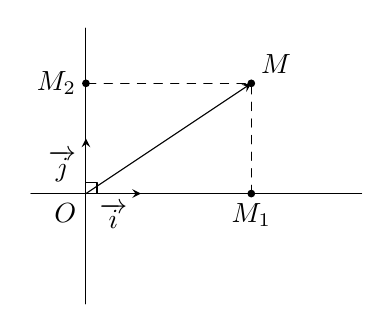
\begin{tikzpicture}[line cap=round,line join=round,>=stealth,x=1.0cm,y=1.0cm,scale=.7]
	\draw(0,-2)--(0,3) (-1,0)--(5,0);
	\draw[->] (0,0)--(0,1);
	\draw[->] (0,0)--(1,0);
	\draw[->] (0,0) -- (3,2);
	\draw (0,0) node [below left] {$ O $} (0,2) node [left] {$ M_2 $} (3,0) node [below] {$ M_1 $} (3,2) node [above right] {$ M $};
	\draw(0,0.5) node [left] {$ \overrightarrow{j} $};
	\draw (0.5,0) node[below] {$ \overrightarrow{i} $};	
	:\fill (0,2) circle (2pt) (3,0) circle (2pt) (3,2) circle (2pt);
	\draw[dashed] (3,0)--(3,2)--(0,2) ;
	\draw (0,0) rectangle (0.2,0.2);
	\end{tikzpicture} 
	}		
		$$M=(x;y)\Leftrightarrow\overrightarrow{OM}=x\overrightarrow{i}+y\overrightarrow{j}.$$		
	\textbf{Chú ý rằng:} nếu $MM_1\perp Ox$, $MM_2\perp Oy$ thì $x=\overline{OM}_1$, $y=\overline{OM}_2$.
\end{enumerate}
\subsubsection{BIỂU THỨC TỌA ĐỘ CỦA PHÉP TOÁN VÉC-TƠ}
	\begin{dl}
		Cho $\overrightarrow{u}=(x;y)$; $\overrightarrow{u}'=(x’;y’)$ và số thực $k$. Khi đó, ta có
		\begin{enumerate}
			\item  $\overrightarrow{u}=\overrightarrow{u}'\Leftrightarrow\heva{&x=x’\\&y=y’.}$ 
			\item  $\overrightarrow{u}\pm\overrightarrow{v}=(x\pm x’;y\pm y’)$.
			\item  $k\cdot\overrightarrow{u}=(kx;ky)$.
			\item  $\overrightarrow{u’}$ cùng phương $\overrightarrow{u}$ ($\overrightarrow{u}\neq\overrightarrow{0}$) khi và chỉ khi có số $k$ sao cho $\heva{&x’=kx\\&y’=ky.}$ 
			\item  Cho $A(x_A;y_A)$, $B(x_B;y_B)$ thì $\overrightarrow{AB}=\left(x_B-x_A;y_B-y_A\right)$. Khi đó, độ dài của đoạn thẳng $AB=\left|\overrightarrow{AB}\right|=\sqrt{\left(x_B-x_A\right)^2+\left(y_B-y_A\right)^2}$.
		\end{enumerate}		
	\end{dl}
\subsubsection{TỌA ĐỘ TRUNG ĐIỂM CỦA ĐOẠN THẲNG - TỌA ĐỘ TRỌNG TÂM CỦA TAM GIÁC}
\begin{enumerate}	
\item \textbf{Tọa độ trung điểm của đoạn thẳng}\\
Cho đoạn thẳng $AB$ có $A(x_A;y_A)$, $B(x_B;y_B)$. Ta dễ dàng chứng minh được tọa độ trung điểm $I(x_I;y_I)$ của đoạn thẳng $AB$ là $$x_I=\dfrac{x_A+x_B}{2}, y_I=\dfrac{y_A+y_B}{2}.$$
\item \textbf{Tọa độ trọng tâm của tam giác}\\
Cho tam giác $ABC$ có $A(x_A;y_A)$, $B(x_B;y_B), C(x_C;y_C)$. Khi đó tọa độ của trọng tâm $G(x_G;y_G)$ của tam giác $ABC$ được tính theo công thức $$x_G=\dfrac{x_A+x_B+x_C}{3}, y_G=\dfrac{y_A+y_B+y_C}{3}.$$
\end{enumerate}	
\end{tomtat}
\subsection{Các ví dụ}
\begin{vd}%Ví dụ 1%[0H1Y4-3]
	Trên trục tọa độ $\left(O;\overrightarrow{i}\right)$ cho 2 điểm $A$, $B$ có tọa độ lần lượt là $-2; 1$. Tìm tọa độ của vectơ $\overrightarrow{AB}$.
	\loigiai{
Ta có  $\overrightarrow{AB}=1+2=3$.	Vậy toạ độ $\overrightarrow{AB} $ là $3$.
	}
\end{vd}

\begin{vd}%Ví dụ 1%[0H1BY4-3]
Trong mặt phẳng tọa độ $Oxy$. Cho điểm $M(x;y)$. Tìm tọa độ của các điểm $M_1$ đối xứng với $M$ qua trục hoành.
	\loigiai{
	$M_1$ đối xứng với $M$ qua trục hoành suy ra $M_1(x;-y)$.}
\end{vd}
\begin{vd}%Ví dụ 2%[0H1Y4-3]
	Trong mặt phẳng $Oxy$, cho hai điểm $A(1; 2)$, $B(-2; 3)$. Tìm tọa độ của vectơ $\overrightarrow{AB}$.
	\loigiai{
		Ta có $\overrightarrow{AB}=(-2-1; 3-2)=(-3; 1)$.}
\end{vd}
\begin{vd}%Ví dụ 3%[0H1Y4-4]%[Nguyen Tam Phuc]
	Vectơ $\overrightarrow{a}=(-4;0)$ được phân tích theo hai vectơ đơn vị $\left(\overrightarrow{i};\overrightarrow{j}\right)$ như thế nào?
	\loigiai{
		Ta có $\overrightarrow{a}=(-4;0)\Rightarrow\overrightarrow{a}=-4\overrightarrow{i}+0\overrightarrow{j}=-4\overrightarrow{i}$.}
\end{vd}
\begin{vd}%Ví dụ 4%[0H1K4-3]
	Trong hệ trục tọa độ $Oxy$, cho hình vuông $ABCD$ tâm $I$ và có $A(1;3)$. Biết điểm $B$ thuộc trục $Ox$ và $\overrightarrow{BC}$ cùng hướng với $\overrightarrow{i}$. Tìm tọa độ vectơ $\overrightarrow{AC}$.
	\loigiai{
		\immini{Từ giả thiết ta xác định được hình vuông trên mặt phẳng tọa độ $Oxy$ như hình vẽ bên.\\
		Vì điểm $A(1;3)$ suy ra $AB=3$, $OB=1$.\\
		Do đó $B(1;0)$, $C(4;0)$, $D(4;3)$.\\
		Vậy $\overrightarrow{AC}=(3;-3)$.
	}{
		\begin{tikzpicture}[line cap=round,line join=round,>=stealth,x=1.0cm,y=1.0cm,scale=.8]
		\def\xmin{-1}
		\def\xmax{5}
		\def\ymin{-1}
		\def\ymax{4}
		\tikzset{label style/.style={font=\footnotesize}}
		\draw[->] (\xmin,0)--(\xmax,0) node[below left] {$x$};
		\draw[->] (0,\ymin)--(0,\ymax) node[below left] {$y$};
		\draw (0,0) node [below left] {$O$};
		\begin{scope}
		\clip (\xmin,\ymin) rectangle (\xmax,\ymax); 
		\path 
		(1,3) coordinate (A)
		(1,0) coordinate (B)	
		(4,0) coordinate (C)	
		(4,3) coordinate (D)	
		($(A)!0.5!(C)$) coordinate (O)	
		;
		
		\foreach \x/\g in{A/90,B/-90,C/-90,D/90,O/90}
		\fill[black](\x) circle (2pt)
		($(\x)+(\g:3mm)$) node{\small $\x$};
		\end{scope}
		\draw (A)--(B)--(C)--(D)--(B) (A)--(C) (A)--(D);
		\draw[dashed] (0,3)--(1,3);
		\fill (0,1) node [left] {$ 1 $} circle (1pt) (0,2) node [left] {$ 2 $} circle (1pt) (0,3) node [left] {$ 3 $} circle (1pt) (2,0) node [below] {$ 2 $} circle (1pt) (3,0) node [below] {$ 3 $} circle (1pt) ;
		\end{tikzpicture} 
	}
	}
\end{vd}
\begin{vd}%[0H1Y4-2]
	Trong mặt phẳng $Oxy$, cho hai vectơ $\overrightarrow{a}=(1;3)$, $\overrightarrow{b}=(3;-4)$. Tìm tọa độ vectơ $\overrightarrow{a}-\overrightarrow{b}$.
	\loigiai{
		Ta có $\overrightarrow{a}-\overrightarrow{b}=\left(1-3; 3-(-4)\right)=(-2;7)$.}
\end{vd}
\begin{vd}%[0H1Y4-2]
	Trong mặt phẳng $Oxy$, cho $\overrightarrow{a}=(x;2)$, $\overrightarrow{b}=(-5;1)$, $\overrightarrow{c}=(x;7)$. Tìm $x$ để vectơ $\overrightarrow{c}=2\overrightarrow{a}+3\overrightarrow{b}$.
	\loigiai{
		Ta có $\overrightarrow{c}=2\overrightarrow{a}+3\overrightarrow{b}$ $\Rightarrow x=2\cdot x+3\cdot (-5)\Leftrightarrow x=15$.}
\end{vd}
\begin{vd}%[0H1B4-3]
	Trong mặt phẳng $Oxy$, cho hai điểm $A(1;0)$ và $B(0;-2)$. Tọa độ điểm $D$ sao cho $\overrightarrow{AD}=-3\overrightarrow{AB}$ là
	\loigiai{
		Ta có $\overrightarrow{AD}=-3\overrightarrow{AB}$ $\Leftrightarrow \heva{&x_D-1=-3(0-1)\\&y_D-0=-3(-2-0)}\Leftrightarrow\heva{&x_D=4\\&y_D=6}\Rightarrow D(4; 6)$.}
\end{vd}


\subsection{Các dạng toán thường gặp}

\begin{dang}{Tọa độ của điểm và độ dài đại số của một vectơ trên trục}
    \begin{itemize}
        \item Điểm $M$ có tọa độ $a \Leftrightarrow \vec{OM}=a.\vec{e}$ với $O$ là điểm gốc.
        \item vectơ $\vec{AB}$ có độ dài đại số là $m=\overline{AB}\Leftrightarrow \vec{AB}=m\vec{e}$.
        \item Nếu $A$ và $B$ có tọa độ lần lượt là $a$ và $b$ thì $\overline{AB}=b-a$.
        \item Tọa độ trung điểm $I$ của đoạn $AB: x_I=\dfrac{x_A + x_B}{2}$.
    \end{itemize}
\end{dang}

\begin{vd}%[Hồng Trường Sơn]%[0H1B4-1]
    Trên trục tọa độ $(O;\vec{e})$, cho ba điểm $A$, $B$, $C$ với $\vec{OA}=4{,}5\vec{e}$, $\vec{OB}=-7{,}2\vec{e}$, $\vec{OC}=-3{,}6\vec{e}$.
    \begin{enumerate}[a)]
        \item Xác định tọa độ các điểm $A$, $B$, $C$.
        \item Tìm tọa độ các trung điểm $M$, $N$, $P$ theo thứ tự của các đoạn thẳng $AB$, $BC$, $CA$.
        \item Tính độ dài các đoạn thẳng $AB$, $BC$, $CA$.
    \end{enumerate}
    \loigiai{
        \begin{center}
            \begin{tikzpicture}
            \draw[->] (-8.5,0) -- (5.5,0);
            \foreach \x in {}
            \draw[shift={(\x,0)},color=black] (0pt,2pt) -- (0pt,-2pt) node[below] { $\x$};
            \draw[->,line width=1] (0,0) -- (1,0);
            \draw [fill=black] (0,0) circle (1.5pt);
            \draw [fill=black] (-7.2,0) circle (1.5pt);
            \draw [fill=black] (-3.6,0) circle (1.5pt);
            \draw [fill=black] (4.5,0) circle (1.5pt);
            %   \draw[color=black] (5.5,0) node[right] {$x$};
            \draw[color=black] (0,0) node[above] {$O$};
            \draw[color=black] (-7.2,0) node[above] {$B$};
            \draw[color=black] (-7.2,0) node[below] {$-7{,}2$};
            \draw[color=black] (-3.6,0) node[above] {$C$};
            \draw[color=black] (-3.6,0) node[below] {$-3{,}6$};
            \draw[color=black] (4.5,0) node[above] {$A$};
            \draw[color=black] (4.5,0) node[below] {$4{,}5$};
            \draw[color=black] (0.5,0) node[above] {$\vec{e}$};
            \end{tikzpicture}
        \end{center}
    \begin{enumerate}[a)]
        \item Theo định nghĩa tọa độ của điểm trên trục ta có
        \begin{itemize}
            \item Tọa độ của điểm $A$ là $4{,}5$.
            \item Tọa độ của điểm $B$ là $-7{,}2$.
            \item Tọa độ của điểm $B$ là $-3{,}6$.
        \end{itemize}
        \item Vì $M$ là trung điểm $AB\Rightarrow x_M=\dfrac{x_A+x_B}{2}=-1{,}35\Rightarrow M(-1{,}35)$.\\ 
        Tương tự ta được tọa độ điểm $N$ là $-5{,}4$, tọa độ điểm $P$ là $0{,}45$.
        \item $\overline{AB}=-11{,}7\Rightarrow AB=11{,}7$, $\overline{BC}=3{,}6\Rightarrow BC=3{,}6$, $\overline{CA}=8{,}1\Rightarrow CA=8{,}1$.
        \end{enumerate}
    }
\end{vd}
\begin{vd}%[Hồng Trường Sơn]%[0H1B4-1]
    Trên trục $(O; \overrightarrow{e})$, cho các điểm $A$, $B$, $M$, $N$ có tọa độ lần lượt là $-1$, $2$, $3$, $-2$. Tính độ dài đại số của $\overrightarrow{AB}$ và $\overrightarrow{MN}$.
\loigiai{
    \begin{center}
        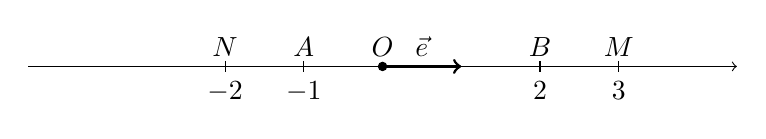
\begin{tikzpicture}
        \draw[->] (-4.5,0) -- (4.5,0);
        \foreach \x in {-2,-1,2,3}
        \draw[shift={(\x,0)},color=black] (0pt,2pt) -- (0pt,-2pt) node[below] { $\x$};
        \draw[->,line width=1] (0,0) -- (1,0);
        \draw [fill=black] (0,0) circle (1.5pt);
        %   \draw[color=black] (5.5,0) node[right] {$x$};
        \draw[color=black] (0,0) node[above] {$O$};
        \draw[color=black] (-1,0) node[above] {$A$};
        \draw[color=black] (-2,0) node[above] {$N$};
        \draw[color=black] (2,0) node[above] {$B$};
        \draw[color=black] (3,0) node[above] {$M$};
        \draw[color=black] (0.5,0) node[above] {$\vec{e}$};
        \end{tikzpicture}
    \end{center}
$\overline{AB}=b-a=2-(-1)=3$.\\
$\overline{MN}=n-m=-2-3=-5$.
}
\end{vd}
\begin{vd}%[Hồng Trường Sơn]%[0H1B4-1]
    Trên trục tọa độ $\left(O,\vec{e}\right)$, cho ba điểm $A$, $B$, $C$ có tọa độ lần lượt là $1,-2,7$. 
    \begin{enumerate}
        \item Tìm tọa độ điểm $M$ sao cho $\overline{AM}+3\overline{BM}=2\overline{CM}$.
        \item Tìm tọa độ của $D$ sao cho $\overline{DA}+4\overline{DB}\le 3\overline{DC}$.
    \end{enumerate}
    \loigiai{
        \begin{center}
            \begin{tikzpicture}
            \draw[->,color=black] (-3.5,0) -- (8,0);
            \foreach \x in {-2,1,7}
            \draw[shift={(\x,0)},color=black] (0pt,2pt) -- (0pt,-2pt) node[below] { $\x$};
            \draw[->,line width=1] (0,0) -- (1,0);
            \draw [fill=black] (0,0) circle (1.5pt);
            %   \draw[color=black] (8,0) node[right] {$x$};
            \draw[color=black] (0,0) node[above] {$O$};
            \draw[color=black] (-2,0) node[above] {$B$};
            \draw[color=black] (7,0) node[above] {$C$};
            \draw[color=black] (1,0) node[above] {$A$};
            \draw[color=black] (0.5,0) node[above] {$\vec{e}$};
            \end{tikzpicture}
        \end{center}
    \begin{enumerate}
        \item Gọi tọa độ điểm $M$ là $x$, ta có $\overline{AM}=x-1$, $\overline{BM}=x+2$, $\overline{CM}=x-7$. \\
        Theo giả thiết ta suy ra $x-1+3(x+2)=3(x-7)\Leftrightarrow x=-26$.
        \item Gọi tọa độ điểm $D$ là $x$, ta có $\overline{DA}=1-x$, $4\overline{DB}=-8-4x$, $3\overline{DC}=21-3x$. \\
        Theo giả thiết ta suy ra $1-x-8-4x \le 21-3x \Rightarrow x \ge -14$.
    \end{enumerate}
    }
\end{vd}


\begin{dang}{Tọa độ của điểm và của vectơ}
    \begin{itemize}
    \item Áp dụng định nghĩa tọa độ của điểm.
    \item Áp dụng định nghĩa tọa độ của vectơ.
    \item Sử dụng các tính chất của phép toán vectơ.
\end{itemize}
\end{dang}
\begin{vd}%[Hồng Trường Sơn]%[0H1B4-2]
    Trong mặt phẳng $(Oxy)$, tìm tọa độ của các vectơ sau?
    \begin{listEX}[2]
        \item $\overrightarrow{u}=2\overrightarrow{i}+3\overrightarrow{j}$.
        \item $\overrightarrow{v}=\pi\overrightarrow{i}-\sqrt{3}\overrightarrow{j}$.
        \item $\overrightarrow{x}=-3\overrightarrow{j}$.
        \item $\overrightarrow{u}=\sqrt{2}\overrightarrow{i}$.
    \end{listEX}
\loigiai{
Áp dụng định nghĩa tọa độ của vectơ, ta có
\begin{listEX}[2]
    \item $\overrightarrow{u}=\left(2;3\right)$.
    \item $\overrightarrow{v}=\left(\pi;-\sqrt{3}\right)$.
    \item $\overrightarrow{x}=\left(0;-3\right)$.
    \item $\overrightarrow{u}=\left(\sqrt{2};0\right)$.
\end{listEX}
}
\end{vd}
\begin{vd}%[Hồng Trường Sơn]%[0H1B4-2]
    Trong mặt phẳng $(Oxy)$, tìm tọa độ của các điểm thỏa mãn?
    \begin{listEX}[2]
        \item $\overrightarrow{OM}=-2\overrightarrow{i}+\overrightarrow{j}$.
        \item $\overrightarrow{ON}=-3\overrightarrow{i}+4\overrightarrow{j}$.
        \item $\overrightarrow{OP}=2\overrightarrow{j}$.
        \item $\overrightarrow{OQ}=-5\overrightarrow{i}$.
    \end{listEX}
\loigiai{
Áp dụng định nghĩa tọa độ của điểm, ta có
\begin{listEX}[2]
    \item $\overrightarrow{OM}=\left(-2;1\right) \Leftrightarrow M\left(-2;1\right)$.
    \item $\overrightarrow{ON}=\left(-3;4\right) \Leftrightarrow N\left(-3;4\right)$.
    \item $\overrightarrow{OP}=\left(0;2\right) \Leftrightarrow P\left(0;2\right)$.
    \item $\overrightarrow{OQ}=\left(-5;0\right) \Leftrightarrow Q\left(-5;0\right)$.
\end{listEX}
}
\end{vd}
\begin{vd}%[Hồng Trường Sơn]%[0H1B4-2]
\immini{
Trong mặt phẳng tọa độ $Oxy$, cho $\overrightarrow{u}$ như hình vẽ bên. Xác định tọa độ của $\overrightarrow{u}$.
}{
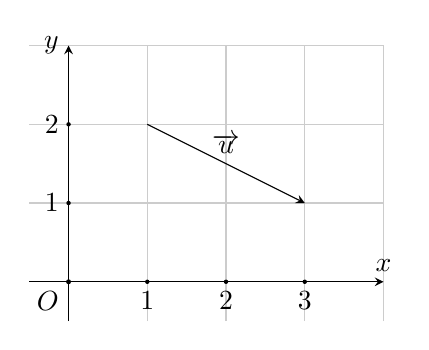
\begin{tikzpicture}
\draw[gray!40] (-0.5,-0.5) grid (4,3);
\draw[-stealth] (-0.5,0)--(4,0) node[above]{$x$};
\draw[-stealth](0,-0.5) --(0,3) node[left]{$y$};
\fill
(0,0) circle (0.9pt) node [below left]{$O$}
(1,0) circle (0.8pt) node [below]{$1$}
(2,0) circle (0.8pt) node [below]{$2$}
(0,1) circle (0.8pt) node [left]{$1$}
(0,2) circle (0.8pt) node [left]{$2$}
(3,0) circle (0.8pt) node [below]{$3$}
; 
\draw[-stealth]  (1,2)--(3,1) node[pos=0.5,above]{$\overrightarrow{u}$};
\end{tikzpicture}
}
\loigiai{
\begin{center}
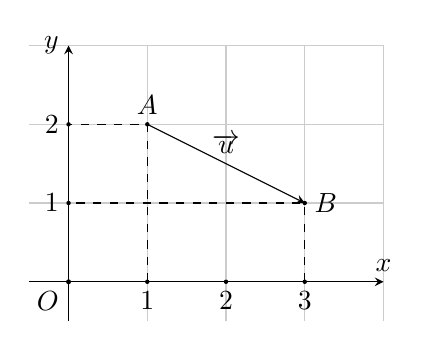
\begin{tikzpicture}
\draw[gray!40] (-0.5,-0.5) grid (4,3);
\draw[-stealth] (-0.5,0)--(4,0) node[above]{$x$};
\draw[-stealth](0,-0.5) --(0,3) node[left]{$y$};
\fill
(0,0) circle (0.9pt) node [below left]{$O$}
(1,0) circle (0.8pt) node [below]{$1$}
(2,0) circle (0.8pt) node [below]{$2$}
(0,1) circle (0.8pt) node [left]{$1$}
(0,2) circle (0.8pt) node [left]{$2$}
(3,0) circle (0.8pt) node [below]{$3$}
(1,2) circle(0.8pt) node[above]{$A$}  
(3,1) circle(0.8pt) node[right]{$B$}; 
\draw[dashed](1,0)|-(0,2) (3,0)|-(0,1);
\draw[-stealth]  (1,2)--(3,1) node[pos=0.5,above]{$\overrightarrow{u}$};
\end{tikzpicture}
\end{center}
\begin{itemize}
    \item Dựa vào hình vẽ, ta có điểm đầu của $\overrightarrow{u}$ là $A(1;2)$ và điểm cuối của $\overrightarrow{u}$ là $B=(3;1)$.
    \item $\overrightarrow{u}=\overrightarrow{AB}=(3-1;1-2)=(2;-1)$.
\end{itemize}
}
\end{vd}
\begin{vd}%[Hồng Trường Sơn]%[0H1B4-2]
    Trong mặt phẳng tọa độ $Oxy$, cho $\overrightarrow{a}=(2;-1)$, $\overrightarrow{b}=(-1;-4)$ và $\overrightarrow{c}=(-3;2)$. 
    \begin{listEX}
        \item Tìm tọa độ của $\overrightarrow{u}=2\overrightarrow{a}+3\overrightarrow{b}$.
        \item Tìm tọa độ của $\overrightarrow{x}=4\overrightarrow{a}+7\overrightarrow{b}-2\overrightarrow{c}$.
    \end{listEX}
\loigiai{
\begin{enumerate}
    \item Ta có $2\overrightarrow{a}=(4;-2)$ và $3\overrightarrow{b}=(-3;-12)$.\\
    $\Rightarrow \overrightarrow{u}=2\overrightarrow{a}+3\overrightarrow{b}=(4+(-3);-2+(-12)) =(1;-14)$.\\ 
    Vậy $\overrightarrow{u}=(1;-14)$.
    \item Ta có $4\overrightarrow{a}=(8;-4)$, $7\overrightarrow{b}=(-7;-28)$ và $-2\overrightarrow{c}=(6;-4)$.\\
    $\Rightarrow \overrightarrow{x}=4\overrightarrow{a}+7\overrightarrow{b}-2\overrightarrow{c}=(8+(-7)+6;-4+(-28)+(-4)) =(7;-36)$.\\
    Vậy $\overrightarrow{x}=(7;-36)$.
\end{enumerate}
}
\end{vd}
\begin{dang}{Tọa độ của điểm và vectơ thỏa mãn điều kiên cho trước}
    \textbf{Phương pháp}
    \begin{itemize}
        \item Gọi điểm (vectơ) cần tìm có tọa độ $(x;y)$.
        \item Theo yêu cầu bài toán, lập hệ phương trình với hai ẩn $x,y$.
        \item Giải hệ phương trình tìm $x,y \Rightarrow$ tọa độ của điểm (vectơ) cần tìm.
    \end{itemize}
\end{dang}

\begin{vd}%[Hồng Trường Sơn]%[0H1B4-3]
    Trong mặt phẳng $Oxy$, cho ba điểm $A(1;-2)$, $B(3;4)$, $C(-2;-1)$. 
    \begin{enumerate}
        \item Tìm tọa độ trung điểm của cạnh $AB$.
        \item Tìm tọa độ trọng tâm của tam giác $ABC$.
        \item Tìm tọa độ điểm $D$ sao cho $ABCD$ là hình bình hành.
    \end{enumerate}
    \loigiai{
    \begin{enumerate}
        \item Tọa độ trung điểm $M$ của cạnh $AB$ là $\heva{&x_M= \dfrac{1+3}{2}=2\\ &y_M= \dfrac{-2+4}{2}=1} \Rightarrow M(2;1)$.
        \item Tọa độ trọng tâm $G$ của tam giác $ABC$ là $\heva{&x_G= \dfrac{1+3-2}{3}= \dfrac{2}{3}\\ &y_G= \dfrac{-2+4-1}{3}= \dfrac{1}{3}} \Rightarrow G\left(\dfrac{2}{3};\dfrac{1}{3}\right)$.
        \item Gọi $D\left(x;y\right) \Rightarrow \overrightarrow{AD}=\left(x-1;y+2\right)$ và $\overrightarrow{BC}=\left(-5;-5\right)$.\\
        Ta có $ABCD$ là hình bình hành $\Leftrightarrow \overrightarrow{AD}=\overrightarrow{BC}$
        $$\Leftrightarrow \heva{&x-1=-5\\ &y+2=-5}\Leftrightarrow \heva{&x=-4\\ &y=-7} \Leftrightarrow D\left(-4;-7\right).$$
    \end{enumerate}
    }
\end{vd}
\begin{vd}%[Hồng Trường Sơn]%[0H1B4-3]
    Trong mặt phẳng $Oxy$, cho ba điểm $A(2;-2)$, $B(-3;1)$, $C(1;3)$. 
    \begin{enumerate}
        \item Tìm tọa độ điểm $M$ sao cho $\overrightarrow{MB}=-2\overrightarrow{MA}$.
        \item Tìm tọa độ điểm $M$ thỏa mãn $\overrightarrow{MA}+2\overrightarrow{MB}-\overrightarrow{MC}=\overrightarrow{0}$.
    \end{enumerate}
    \loigiai{
    \begin{enumerate}
        \item Gọi $M\left(x;y\right) \Rightarrow \overrightarrow{MB}=\left(-3-x;1-y\right);\overrightarrow{MA}=\left(2-x;-2-y\right)$\\
        Do đó $-2\overrightarrow{MA}=\left(-4+2x;4+2y\right)$.\\
        Mà $\overrightarrow{MB}=-2\overrightarrow{MA} \Leftrightarrow \heva{&-3-x=-4+2x\\ &1-y=4+2y}$ 
        $$\Leftrightarrow \heva{&3x=1\\ &3y=-3} \Leftrightarrow \heva{&x= \dfrac{1}{3}\\ &y=-1} \Rightarrow M \left(\dfrac{1}{3};-1\right).$$
        \item Gọi $M\left(x;y\right) \Rightarrow \overrightarrow{MA}=\left(2-x;-2-y\right); \overrightarrow{MB}=\left(-3-x;1-y\right)$; $\overrightarrow{MC}=\left(1-x;3-y\right)$.\\
        Do đó $\overrightarrow{MA}+2\overrightarrow{MB}-\overrightarrow{MC}=\left(-5-2x;-3-2y\right)$.\\
        Do $\overrightarrow{MA}+2\overrightarrow{MB}-\overrightarrow{MC}=\overrightarrow{0}$ 
        $$\Leftrightarrow \heva{&-5-2x=0\\ &-3-2y=0}\Leftrightarrow \heva{&x=-\dfrac{5}{2}\\ &y=-\dfrac{3}{2}} \Leftrightarrow M\left(-\dfrac{5}{2};-\dfrac{3}{2}\right).$$
    \end{enumerate}
    }
\end{vd}
\begin{vd}%[Hồng Trường Sơn]%[0H1B4-3]
    Trong mặt phẳng $Oxy$, cho hai điểm $A(-1;1)$, $D\left(-1;\dfrac{5}{2}\right)$.
\begin{enumerate}
    \item Tìm tọa độ điểm $B$ biết $D$ là trung điểm đoạn $AB$.
    \item Tìm tọa độ điểm $M$ đối xứng với $A$ qua $B$.
\end{enumerate}
\loigiai{
\begin{enumerate}   
    \item Gọi $B\left(x_B;y_B\right)$. Ta có
    $$\heva{&x_D=\dfrac{x_A+x_B}{2}\\ &y_D=\dfrac{y_A+y_B}{2}}\Leftrightarrow \heva{&-1=\dfrac{-1+x_B}{2}\\ &\dfrac{5}{2}=\dfrac{1+y_B}{2}}\Leftrightarrow\heva{&x_B=-1\\ &y_B=4.}$$
    Vậy $B\left(-1;4\right)$.
    \item Gọi $M\left(x_M;y_M\right)$ là điểm đối xứng với $A$ qua $B$, khi đó $B$ là trung điểm của $MA$. Ta có
    $$\heva{&x_M=2x_B-x_A\\ &y_M=2y_B-y_A}\Leftrightarrow \heva{&x_M=2.(-1)-(-1)\\ &y_M=2.4-1}\Leftrightarrow\heva{&x_M=-1\\ &y_M=7.}$$
    Vậy $M\left(-1;7\right)$.
\end{enumerate}
}
\end{vd}
\begin{vd}%[Hồng Trường Sơn]%[0H1B4-3]
    Trong mặt phẳng tọa độ $Oxy$, cho các vectơ $\overrightarrow{a}=(x;2), \overrightarrow{b}=(-5;1)$ và \break $\overrightarrow{c}=(x;7)$. Tìm $x$ sao cho $\overrightarrow{c}=2\overrightarrow{a}+3\overrightarrow{b}$.
\loigiai{
\begin{itemize}
    \item $2\overrightarrow{a}=2(x;2)=(2x;4)$.
    \item $3\overrightarrow{b}=3(-5;1)=(-15;3)$.
    \item $\overrightarrow{c}=2\overrightarrow{a}+3\overrightarrow{b} =(2x-15;7)\Leftrightarrow (x;7)=(2x-15;7) \Leftrightarrow \heva{x &=2x-15 \\ 7&= 7} \Leftrightarrow x =15.$
\end{itemize}
Vậy $x=15$.
}
\end{vd}
\begin{vd}%[Hồng Trường Sơn]%[0H1B4-3]
    Trong mặt phẳng $Oxy$, cho $\vec{a}=\left(2; 1\right), \vec{b}=\left(3; 4\right), \vec{c}=\left(7; 2\right)$.
    \begin{enumerate}
        \item Tìm tọa độ của vectơ $\vec{u}=2\vec{a} - 3\vec{b} + \vec{c}$. 
        \item Tìm tọa độ của vectơ $\vec{v}$ sao cho $\vec{v} + \vec{a}=\vec{b} - \vec{c}$. 
        \item Tìm các số $k, h$ để $\vec{c}=k\vec{a} + h\vec{b}$. 
    \end{enumerate}
    \loigiai{
    \begin{enumerate}
        \item $\vec{u}=2\vec{a} - 3\vec{b} + \vec{c}=\left(4; 2\right) - \left(9; 12\right) + \left(7; 2\right)=(2; - 8)$.
        \item $\vec{v} + \vec{a}=\vec{b} - \vec{c}\Leftrightarrow \vec{v}= - \vec{a} + \vec{b} - \vec{c}=(- 6; 1)$.
        \item $\vec{c}=k\vec{a} + h\vec{b} \Leftrightarrow \heva{&7=2k + 7h \\ &2=k + 4h} \Leftrightarrow \heva{&k=\dfrac{22}{5} \\ &h= - \dfrac{3}{5}.}$\\
        Suy ra $ \vec{c}=\dfrac{22}{5}\vec{a} - \dfrac{3}{5}\vec{b}$. 
        \end{enumerate} 
}   
\end{vd}
\begin{dang}{Phân tích một vectơ theo hai vectơ không cùng phương}
    Phân tích $\vec{u}$ theo hai véc tơ không cùng phương $\vec{a}$ và $\vec{b}$.\\
    \textbf{Phương pháp}
    \begin{itemize}
        \item Giả sử $\vec{u}=m\vec{a}+n\vec{b}$.
        \item Lập hệ phương trình với hai ẩn $m,n$.
        \item Giải hệ phương trình tìm $m,n \Rightarrow$ kết luận.
    \end{itemize}
\end{dang}
\begin{vd}%[Hồng Trường Sơn]%[0H1B4-4]
    Trong mặt phẳng $Oxy$, cho các vectơ $\vec{a}=(4; - 2), \vec{b}=\left(- 1; - 1\right), \vec{c}=\left(2; 5\right)$. 
    \begin{enumerate}
        \item Tìm tọa độ vectơ $\vec{u}=2\vec{a}+3\vec{b}-\vec{c}$.
        \item Hãy phân tích vectơ $\vec{b}$ theo hai vectơ $\vec{a}$ và $\vec{c}$.
    \end{enumerate}
    \loigiai{
    \begin{enumerate}
        \item Ta có $2\vec{a}=(8;-4); 3\vec{b}=(-3;-3); -\vec{c}=(-2;-5)$.
        $$\Rightarrow \vec{u}=2\vec{a}+3\vec{b}-\vec{c}= (8-3-2;-4-3-5)=(3;-12).$$
        Vậy $\vec{u}=(3;-12)$.
        \item Giả sử $\vec{b}=m\vec{a} + n\vec{c}\Leftrightarrow \heva{  - 1&=4m + 2n \\    - 1&= - 2m + 5n } \Leftrightarrow \heva{  m&= - \dfrac{1}{8} \\   n&= - \dfrac{1}{4}. } $\\
        Vậy $\vec{b}= - \dfrac{1}{8}\vec{a} - \dfrac{1}{4}\vec{c}$.
    \end{enumerate}
    }
\end{vd}
\begin{vd}%[Hồng Trường Sơn]%[0H1B4-4]
    Trong mặt phẳng $Oxy$, cho $\vec{a}=\left(-2; 1\right), \vec{b}=\left(1; -3\right), \vec{c}=\left(-1; -7\right)$.
    \begin{enumerate}
        \item Tìm các số $k, h$ để $\vec{a}=k\vec{b} + h\vec{c}$. 
        \item Phân tích $\vec{c}$ theo hai vectơ $\vec{a}$ và $\vec{b}$.
    \end{enumerate}
    \loigiai{
    \begin{enumerate}
        \item $\vec{a}=k\vec{b} + h\vec{c} \Leftrightarrow \heva{&-2=k -h\\ &1=-3k -7h} \Leftrightarrow \heva{&k=-\dfrac{3}{2}\\ &h= \dfrac{1}{2}.}$\\ 
        Suy ra $\vec{a}=-\dfrac{3}{2}\vec{b} + \dfrac{1}{2}\vec{c}$. 
        \item Giả sử $\vec{c}=m\vec{a} + n\vec{b} \Leftrightarrow \heva{&-1=-2m+n\\ &-7=m-3n} \Leftrightarrow \heva{&m=2\\ &n=3.}$\\
        Suy ra $\vec{c}=2\vec{a} + 3\vec{b}$. 
    \end{enumerate} 
}   
\end{vd}
\begin{vd}%[Hồng Trường Sơn]%[0H1B4-4]
    Trong mặt phẳng $Oxy$, cho $A\left(-3; 1\right), B\left(-1; 3\right), C\left(1; -1\right)$. Gọi $M$ là điểm thuộc $BC$ sao cho $\overrightarrow{MB}=-2 \overrightarrow{BC}$ và $G$ là trọng tâm của tam giác $ABC$.
    \begin{enumerate}
        \item Phân tích $\overrightarrow{AM}$ theo hai vectơ $\overrightarrow{AB}$ và $\overrightarrow{AC}$. 
        \item Phân tích $\overrightarrow{GM}$ theo hai vectơ $\overrightarrow{AB}$ và $\overrightarrow{AC}$.
    \end{enumerate}
    \loigiai{
    \begin{enumerate}
        \item Gọi $M(x;y) \Rightarrow \overrightarrow{MB}=(-1-x;3-y); \overrightarrow{BC}=(2;-4); \overrightarrow{AB}=(2;2); \overrightarrow{AC}=(4;-2)$.\\
        Mà $\overrightarrow{MB}=-2 \overrightarrow{BC} \Leftrightarrow \heva{&-1-x=-4\\ &3-y=8} \Leftrightarrow \heva{&x=3\\ &y=-5} \Rightarrow M(3;-5) \Rightarrow \overrightarrow{AM}=(6;-6)$.\\
        Giả sử $\overrightarrow{AM} = m\overrightarrow{AB}+n\overrightarrow{AC} \Leftrightarrow \heva{&6=2m+4n\\ &-6=2m-2n} \Leftrightarrow \heva{&m= -1\\&n=2.}$\\
        Vậy $\overrightarrow{AM} = -\overrightarrow{AB}+2\overrightarrow{AC}$.
        \item Ta có tọa độ trọng tâm $G(-1;1) \Rightarrow \overrightarrow{GM}=(4;-6)$.\\
        Giả sử $\overrightarrow{GM} = h\overrightarrow{AB}+k\overrightarrow{AC} \Leftrightarrow \heva{&4=2h+4k\\ &-6=2h-2k} \Leftrightarrow \heva{&h= -\dfrac{4}{3}\\ &k= \dfrac{5}{3}.}$\\
        Vậy $\overrightarrow{GM} = -\dfrac{4}{3}\overrightarrow{AB}+\dfrac{5}{3}\overrightarrow{AC}$.
    \end{enumerate} 
    \textit{\textbf{Chú ý:} Chúng ta hoàn toàn có thể sử dụng cách biến đổi vectơ để thực hiện việc biểu diễn $\overrightarrow{AM},\overrightarrow{GM}$ theo hai vectơ $\overrightarrow{AB}$ và $\overrightarrow{AC}$.}
}   
\end{vd}
\begin{dang}{Chứng minh ba điểm thẳng hàng, vectơ cùng phương, hai đường thẳng song song}
    Sử dụng các điều kiện cần và đủ sau
    \begin{itemize}
        \item Hai vectơ $\vec{a}$ và $\vec{b} \neq \vec{0}$ cùng phương $\Leftrightarrow$ tồn tại số $k$ sao cho $\vec{a}=k\vec{b}$.\\
        Cụ thể, nếu $\vec{a}=(a_1;a_2), \vec{b}=(b_1;b_2)$ thì $\vec{a}=k\vec{b}$ 
        $$\Leftrightarrow \heva{a_1=kb_1 \\a_2=kb_2} \text{ hay } \dfrac{a_1}{b_1}=\dfrac{a_2}{b_2}, b_1b_2 \ne 0.$$
    \item Ba điểm phân biệt $A$, $B$, $C$ thẳng hàng $\Leftrightarrow$ hai vectơ $\vec{AB}$ và $\vec{AC}$ cùng phương.
    \item Điểm $M$ thuộc đường thẳng $AB \Leftrightarrow$ ba điểm $M$, $A$, $B$ thẳng hàng.
    \end{itemize}
\end{dang}
\begin{vd}%[Hồng Trường Sơn]%[0H1B4-5]
Tìm $x$ để các cặp vectơ sau cùng phương
\begin{enumerate}
\item $\vec{a}=(-3;2)$, $\vec{b}=(6;x)$
\item $\vec{m}=(0;4)$, $\vec{n}=(x;7)$
\item $\vec{u}=(x;-6)$, $\vec{v}=(-8;2x)$.
\end{enumerate}
\loigiai
{\begin{enumerate}
\item Để $\vec{a}$ cùng phương với $\vec{b}$ khi và chỉ khi $\dfrac{6}{-3}=\dfrac{x}{2} \Leftrightarrow x=-4$.\\
Vậy $x=-4$.
\item Để $\vec{m}$ cùng phương với $\vec{n}$ khi và chỉ khi $\vec{n}=k\vec{m} \Leftrightarrow \heva{x=k0 \\7=k4} \Leftrightarrow \heva{x=0 \\k=\dfrac{7}{4}}$\\
Vậy $x=0$.
\item Ta có $\vec{u}$ cùng phương với $\vec{v}$ khi $\dfrac{x}{-8}=\dfrac{-6}{2x} \Rightarrow x^2=24 \Rightarrow x=\pm \sqrt{24} \Rightarrow x=\pm 2\sqrt{6}$.\\
Vậy $x=\pm 2\sqrt{6}$.
\end{enumerate}}
\end{vd}
%---------*---------*---------*---------*---------*---------
\begin{vd}%[Hồng Trường Sơn]%[0H1B4-5]
Trong mặt phẳng $Oxy$, cho các điểm $A(2;-5)$, $B(-3;6)$, $C(12;-27)$, $D(m;2)$.
\begin{enumerate}
\item Chứng minh ba điểm $A$, $B$, $C$ thẳng hàng.
\item Xác định $m$ để ba điểm $A$, $B$, $D$ thẳng hàng.
\end{enumerate}
\loigiai
{\begin{enumerate}
\item Ta có $\vec{AB}=(-5;11)$ và $\vec{AC}=(10;-22)$.\\
Vì $\dfrac{-5}{10} = \dfrac{11}{-22} = -\dfrac{1}{2}$ nên hai vectơ $\vec{AB}$ và $\vec{AC}$ cùng phương.\\ 
Do đó, ba điểm $A$, $B$, $C$ thẳng hàng.
\item Ta có $\vec{AB}=(-5;11)$ và $\vec{AD}=(m-2;7)$.\\
Các điểm $A$, $B$, $D$ thẳng hàng khi và chỉ khi $\dfrac{m-2}{-5}=\dfrac{7}{11}$ 
$$\Leftrightarrow 11(m-2)=-5.7 \Leftrightarrow m=-\dfrac{23}{11}.$$
Vậy $m=-\dfrac{23}{11}$.
\end{enumerate}}
\end{vd}
%---------*---------*---------*---------*---------*---------
\begin{vd}%[Hồng Trường Sơn]%[0H1B4-5]
Trong mặt phẳng $Oxy$, cho ba điểm $M(4;0)$, $N(-2;3)$, $P(6;1)$.
\begin{enumerate}
\item Chứng minh ba điểm $M$, $N$, $P$ là ba đỉnh của một tam giác.
\item Xác định điểm $Q$ trên trục hoành biết các điểm $N$, $P$, $Q$ thẳng hàng.
\end{enumerate}
\loigiai
{\begin{enumerate}
\item Ta có $\vec{MN}=(-6;3)$ và $\vec{MP}=(2;1)$.\\
Vì $\dfrac{-6}{2} \neq \dfrac{3}{1}$ nên hai vectơ $\vec{MN}$ và $\vec{MP}$ không cùng phương.\\ 
Do đó, ba điểm $M$, $N$, $P$ không thẳng hàng, chúng là ba đỉnh của tam giác $MNP$.
\item Giả sử $Q(x;0) \in Ox$. Ta có $\vec{NP}=(8;-2)$ và $\vec{NQ}=(x+2;-3)$.\\
Các điểm $N$, $P$, $Q$ thẳng hàng khi và chỉ khi 
$$\dfrac{x+2}{8}=\dfrac{-3}{-2} \Leftrightarrow 2(x+2)=3.8 \Leftrightarrow x=10.$$
Vậy $Q(10;0)$.
\end{enumerate}}
\end{vd}
%---------*---------*---------*---------*---------*---------
\begin{vd}%[Hồng Trường Sơn]%[0H1B4-5]
Trong mặt phẳng $Oxy$, cho hai điểm $A(3;8)$, $B(6;1)$. Tìm $x$ để điểm $C(-9;x)$ thuộc đường thẳng $AB$.
\loigiai
{Điểm $C$ thuộc đường thẳng $AB$ khi và chỉ khi ba điểm $A$, $B$, $C$ thẳng hàng.\\ 
Tức là hai vectơ $\vec{AB}$ và $\vec{AC}$ cùng phương.\\
Ta có $\vec{AB}=(3;-7)$ và $\vec{AC}=(-12;x-8)$.\\
Lại có $\vec{AB}$ và $\vec{AC}$ cùng phương khi và chỉ khi 
$$\vec{AC}=k\vec{AB} \Leftrightarrow \dfrac{-12}{3}=\dfrac{x-8}{-7} \Leftrightarrow x-8=28 \Leftrightarrow x=36.$$
Vậy $x=36$.}
\end{vd}
%---------*---------*---------*---------*---------*---------
\begin{vd}%[Hồng Trường Sơn]%[0H1B4-5]
Trong mặt phẳng $Oxy$, cho bốn điểm $A(3;-4)$, $B(5;0)$, $C(-6;3)$, $D(2;19)$. Chứng minh đường thẳng $AB$ và $CD$ song song.
\loigiai
{Ta có $\vec{AB}=(2;4)$ và $\vec{CD}=(8;16) \Rightarrow \vec{CD}=4\vec{AB}$.\\ 
Do đó hai đường thẳng $AB$ và $CD$ song song hoặc trùng nhau.\\
Mặt khác, $\vec{AC}=(-9;7)$ và $\vec{AB}=(2;4)$ không cùng phương.\\ 
Do đó điểm $C$ không thuộc đường thẳng $AB$.\\
Vậy đường thẳng $AB$ và $CD$ song song.}
\end{vd}
\subsection{Bài tập tự luận}
\begin{bt}
Trong mặt phẳng tọa độ $Oxy$, cho các điểm $M(1;3), N(4;2)$
\begin{listEX}[1]
	\item Tính độ dài các đoạn thẳng $OM, ON, MN$.
	\item Chứng minh rằng tam giác $OMN$ vuông.
\end{listEX}
	\loigiai
	{
	\begin{listEX}[1]
		\item  $\centerdot \, \overrightarrow{OM}=(1;3)\Rightarrow OM=|\overrightarrow{OM}|=\sqrt{1^2+3^2}=\sqrt{10}$.\\
	 $\centerdot \, \overrightarrow{ON}=(4;2)\Rightarrow ON=|\overrightarrow{ON}|=\sqrt{4^2+2^2}=2\sqrt{5}$.\\
	  $\centerdot\, \overrightarrow{MN}=(3;-1)\Rightarrow MN=|\overrightarrow{MN}|=\sqrt{3^2+(-1)^2}=\sqrt{10}$.
		\item  Ta có $OM^2+MN^2=ON^2=20$ suy ra $\triangle OMN$ vuông tại $M$.
\end{listEX}
	}
\end{bt}
\begin{bt}
	Trong mặt phẳng tọa độ $Oxy$, cho các vectơ $\overrightarrow{a}=3\overrightarrow{i}-2\overrightarrow{j}, \overrightarrow{b}=(4;-1)$ và các điểm $M(-3;6), N(3;-3)$.
	\begin{listEX}[1]
		\item Tìm mối liên hệ giữa các vectơ $\overrightarrow{MN}$ và $2\overrightarrow{a}-\overrightarrow{b}$.
		\item Các điểm $O,M,N$ có thẳng hàng hay không?
		\item Tìm điểm $P(x;y)$ để $OMNP$ là hình bình hành.
	\end{listEX}
	\loigiai
	{
		\begin{listEX}[1]
			\item Ta có $\overrightarrow{MN}=(6;-9), 
			 \overrightarrow{a}=(3;-2)\Rightarrow 2\overrightarrow{a}-\overrightarrow{b}=(2;-3)$.\\
			 Suy ra $\overrightarrow{MN} =3(2\overrightarrow{a}-\overrightarrow{b})$.
			\item $\overrightarrow{OM} =(-3;6),\, \overrightarrow{ON}=(3;-3)$. Vì $\overrightarrow{OM}\ne k\overrightarrow{ON}$ với mọi $k\in\mathbb{R}$, nên 3 điểm $O,M,N$ không thẳng hàng.
			\item Ta có $\overrightarrow{OP}=(x;y),\, \overrightarrow{MN}=(6;-9)$.\\ Tứ giác $OMNP$ là hình bình hành khi $\overrightarrow{OP}=\overrightarrow{MN}\Leftrightarrow \heva{& x=6 \\ & y=-9.}$\\
			Vậy $P(6;-9)$.
		\end{listEX}
	}
\end{bt}
\begin{bt}
	Trong mặt phẳng tọa độ $Oxy$, cho các điểm $A(1;3),B(2;4),C(-3;2)$.
	\begin{listEX}[1]
		\item Chứng minh rằng $A,B,C$ là ba đỉnh của một tam giác.
		\item Tìm tọa độ trung điểm $M$ của đoạn thẳng AB.
		\item Tìm tọa độ trọng tâm $G$ của tam giác $ABC$.
		\item Tìm điểm $D(x;y)$ để $O(0;0)$ là trọng tâm của tam giác $ABD$.
	\end{listEX}
	\loigiai
	{
			\begin{listEX}[1]
			\item Ta có $\overrightarrow{AB}=(1;1),\, \overrightarrow{AC}=(-4;-1)$. Vì $\dfrac{1}{-4}\ne \dfrac{1}{-1}$ nên $\overrightarrow{AB}$ và $\overrightarrow{AC}$ không cùng phương, do đó $A,B,C$ là 3 đỉnh của một tam giác.
			\item Tọa độ trung điểm $M$ của đoạn thẳng $AB$ là $M\left(\dfrac{1+2}{3};\dfrac{3+4}{2}\right)=\left(\dfrac{3}{2};\dfrac{7}{2}\right)$.
			\item Tọa độ trọng tâm của $\triangle ABC$ là $G\left(\dfrac{1+2+(-3)}{3};\dfrac{3+4+2}{3}\right)=(0;3)$.
			\item Vì $O(0;0)$ là trọng tâm của $\triangle ABD$ nên
			$\heva{& \dfrac{1+2+x}{3}=0 \\ & \dfrac{3+4+y}{3}=0}\Leftrightarrow \heva{& x=-3 \\ & y=-7.}$\\
			Vậy $D(-3;7)$.
		\end{listEX}
	}
\end{bt}
\begin{bt}
	Sự dịch chuyển của một tàu thủy được thể hiện trên một mặt phẳng tọa độ như sau: Tàu khởi hành từ vị trí $A(1;2)$ chuyển động đều với vận tốc (tính theo giờ) được biểu thị bởi vectơ $\overrightarrow{v}=(3;4)$. Xác định vị trí của tàu (trên mặt phẳng tọa độ) tại thời điểm sau khi khởi hành $1,5$ giờ.
	\loigiai
	{
	Ta có $\overrightarrow{OA}=(1;2)$, sau khoảng thời gian $t$ tàu ở vị trí có tọa độ xác định bởi $$\overrightarrow{OA}+t\overrightarrow{v}=(1+3t;2+4t).$$
	Vậy sau khi khởi hành $1,5$ giờ tàu ở vị trí có tọa độ là $M(1+3\cdot 1,5;2+4\cdot 1,5)=(5,5;8)$.
	}
\end{bt}
\begin{bt}
	Trong hình $4.38$, quân mã đang ở vị trí có tọa độ $(1;2)$. Hỏi sau một nước đi quân mã có thể đến những vị trí nào?
	\begin{center}
	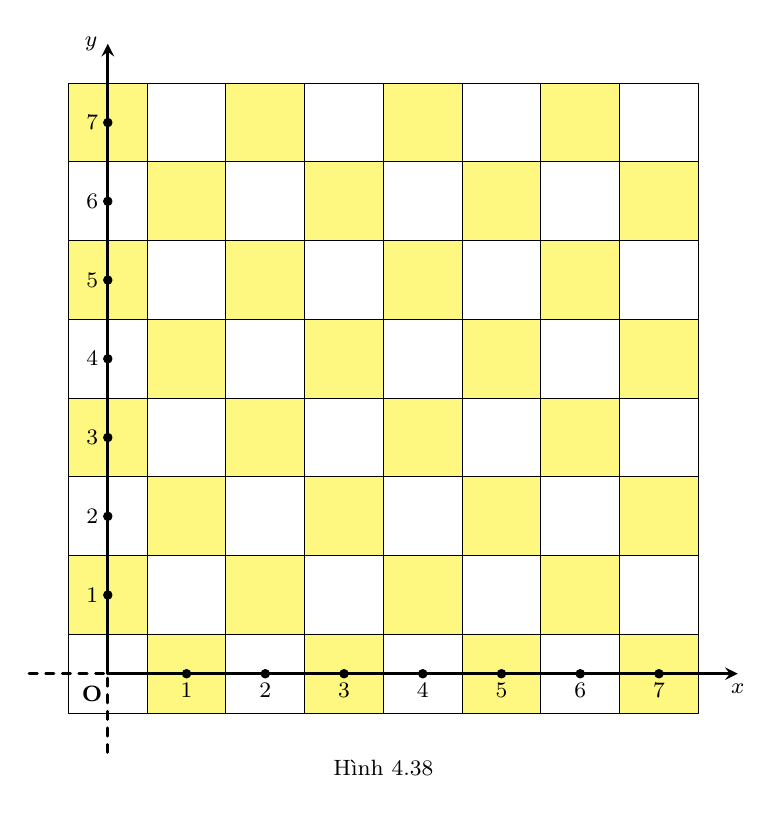
\begin{tikzpicture}[font=\footnotesize, line join=round, line cap=round, >=stealth]
		\begin{scope}
			%Tô màu ô vuông
			\foreach \i in{0,1,...,7}
			\foreach \j in{0,1,...,7}
			{
				\pgfmathparse{mod(\i+\j,2)? "yellow!50": "white"}
				\fill[\pgfmathresult,draw=black](\i,\j)rectangle(\i+1,\j+1);
			}
			\foreach \x/\y/\m in{1/3/\BlackKnightOnWhite,5/4/\BlackRookOnWhite,5/8/\BlackRookOnWhite,7/3/\BlackBishopOnWhite,7/5/\BlackBishopOnWhite
			}
			\path(\x,\y)++(0.5,-0.5)node{\m};
			\foreach \x/\y/\m in{1/6/\BlackKingOnWhite,2/5/\BlackRookOnWhite,3/4/\BlackPawnOnWhite}
			\path(\x,\y)++(0.5,-0.5)node{\color{red}\m};
			\draw[->,line width=1 pt,shift={(0.5,0.5)}](0,0)--(8,0)node[below]{$x$};
			\draw[->,line width=1 pt,shift={(0.5,0.5)}](0,0)--(0,8)node[left]{$y$};
			\foreach \x in {1,2,...,7}{
				\draw[fill=black] (\x,0)++(0.5,0.5)circle(1.5pt)node[below]{$\x$};
				\draw[fill=black] (0.5,\x+0.5)circle(1.5pt)++(0,0)node[left]{$\x$};}
			\draw[dashed,line width=1 pt](-0.5,0.5)--(0.5,0.5)--(0.5,-0.5);
			\node at (4,-0.7){Hình 4.38};
				\node at (0.3,0.25){\textbf{O}};
		\end{scope}
	\end{tikzpicture}
	\end{center}
	\loigiai
	{Quân mã di chuyển theo hình chữ L - hình chữ nhật 2 x 3 hoặc 3 x 2.\\
		Do đó nếu ban đầu quân mã ở vị trí có tọa độ $(1;2)$ thì sau một nước đi  quân mã có thể đến vị trí có tọa độ: $(0;0); (2;0); (3;1); (3;3);(2;4)$ và $(4;0)$.
	}
\end{bt}


\begin{bt}%[0H1Y4-1]
\immini{Tìm tọa độ của các vectơ trong hình bên và biểu diễn mỗi vectơ đó qua vectơ $\vec{i}$ và $\vec{j}$.}
{
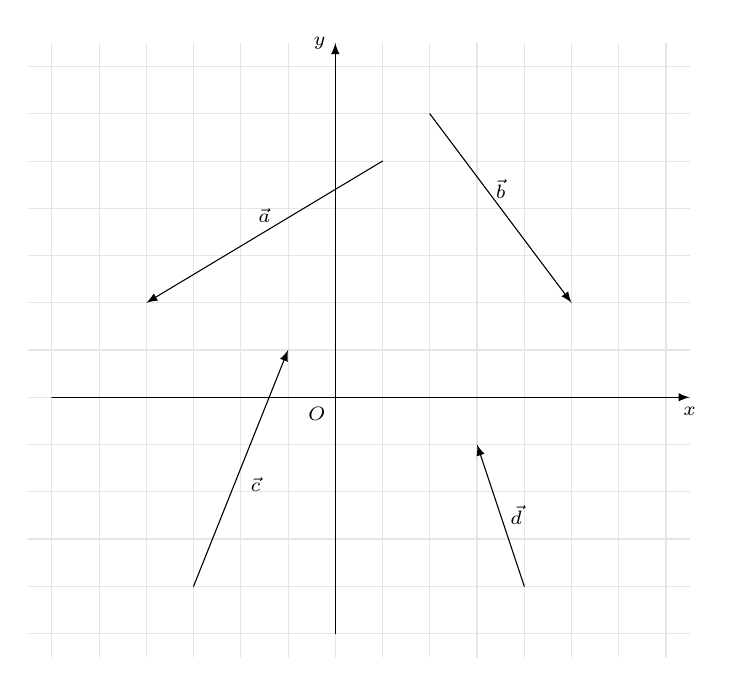
\begin{tikzpicture}[smooth, line join=round, line cap = round, font=\scriptsize,scale=0.6,>=latex]
\draw[gray!20] (-6.5,-5.5) grid (7.5,7.5);
\draw[->] (-6,0) -- (7.5,0) node[below]{$x$};
\draw[->] (0,-5) -- (0,7.5) node[left] {$y$};
\draw (0,0) node[below left] {$O$};
\draw[->] (1,5)--(-4,2);
\draw (-1.5,3.5) node[above]{$\vec{a}$};
\draw[->] (2,6) -- (5,2); 
\draw (3.5,4) node[above]{$\vec{b}$};
\draw[->] (-3,-4)-- (-1,1); 
\draw (-2,-1.5) node[below right] {$\vec{c}$};
\draw[->] (4,-4) -- (3,-1); 
\draw (3.5,-2.5) node[right] {$\vec{d}$};
\end{tikzpicture}
}
	\loigiai{
\begin{center}
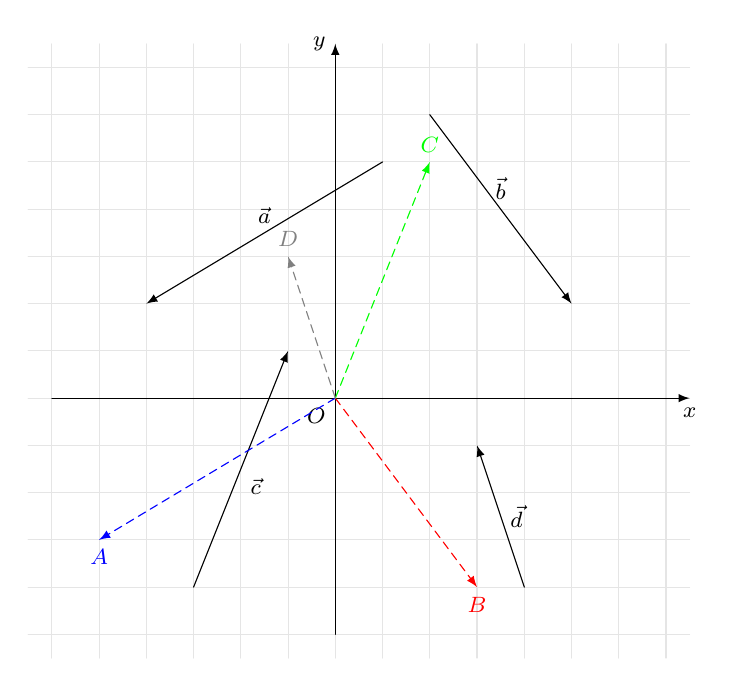
\begin{tikzpicture}[smooth, line join=round, line cap = round, font=\footnotesize,>=latex,scale=0.6]
\draw[gray!20] (-6.5,-5.5) grid (7.5,7.5);
\draw[->] (-6,0) -- (7.5,0) node[below]{$x$};
				\draw[->] (0,-5) -- (0,7.5) node[left] {$y$};
				\draw (0,0) node[below left] {$O$};
				\draw[->] (1,5)--(-4,2);
				\draw (-1.5,3.5) node[above]{$\vec{a}$};
				\draw[->] (2,6) -- (5,2); 
				\draw (3.5,4) node[above]{$\vec{b}$};
				\draw[->] (-3,-4)-- (-1,1); 
				\draw (-2,-1.5) node[below right] {$\vec{c}$};
				\draw[->] (4,-4) -- (3,-1); 
				\draw (3.5,-2.5) node[right] {$\vec{d}$};
				\draw[densely dashed, blue,->] (0,0) -- (-5,-3) node[below]{$A$};
				\draw[densely dashed, red,->] (0,0) -- (3,-4) node[below]{$B$};
				\draw[densely dashed, green,->] (0,0) -- (2,5) node[above]{$C$};
				\draw[densely dashed, gray,->] (0,0) -- (-1,3) node[above]{$D$};
			\end{tikzpicture}
		\end{center}
		\begin{listEX}
			\item Ta có $\vec{a}=\overrightarrow{OA}$ và $A(-5;-3)$, tọa độ vectơ $\overrightarrow{OA}$ chính là tọa độ điểm $A$.\\
			Suy ra $\vec{a}=(-5;-3)$ và $\vec{a}=-5\vec{i}-3\vec{j}$.
			\item Ta có $\vec{b}=\overrightarrow{OB}$ và $B(3,-4)$, tọa độ vectơ $\overrightarrow{OB}$ chính là tọa độ điểm $B$.\\
			Suy ra $\vec{b}=(3;-4)$ và $\vec{b}=3\vec{i}-4\vec{j}$.
			\item Ta có $\vec{c}=\overrightarrow{OC}$ và $C(2,5)$, tọa độ vectơ $\overrightarrow{OC}$ chính là tọa độ điểm $C$.\\
			Suy ra $\vec{b}=(2;5)$ và $\vec{c}=2\vec{i}+5\vec{j}$.
			\item Ta có $\vec{d}=\overrightarrow{OD}$ và $B(-1,3)$, tọa độ vectơ $\overrightarrow{OD}$ chính là tọa độ điểm $D$.\\
			Suy ra $\vec{d}=(-1;3)$ và $\vec{d}=-\vec{i}+3\vec{j}$.
		\end{listEX}
	}
\end{bt}

\begin{bt}%[0H1Y4-1]
	Tìm tọa độ của các vectơ sau
	\begin{enumEX}[a)]{4}
		\item $\vec{a}=3\vec{i}$.
		\item $\vec{b}=-\vec{j}$.
		\item $\vec{c}=\vec{i}-4\vec{j}$.
		\item $\vec{d}=0,5\vec{i}+\sqrt{6}\vec{j}$.
	\end{enumEX}
	\loigiai{
		\begin{enumEX}[a)]{2}
			\item $\vec{a}=3\vec{i}\Rightarrow \vec{a}=(3;0)$.
			\item $\vec{b}=-\vec{j}\Rightarrow \vec{b}=(0;-1)$.
			\item $\vec{c}=\vec{i}-4\vec{j}\Rightarrow \vec{c}=(1;-4)$.
			\item $\vec{d}=0,5\vec{i}+\sqrt{6}\vec{j}\Rightarrow \vec{d}=(0.5,\sqrt{6})$.
		\end{enumEX}
	}
\end{bt}

\begin{bt}%[0H1Y4-3]
	Trong mặt phẳng tọa độ $Oxy$, cho ba điểm $A(2;3)$, $B(-1;1)$, và $C(3;-1)$.
	\begin{listEX}
		\item Tìm tọa độ điểm $M$ sao cho $\overrightarrow{AM}=\overrightarrow{BC}$.
		\item Tìm tọa độ trung điểm $N$ của đoạn thẳng $AC$. Chứng minh $\overrightarrow{BN}=\overrightarrow{NM}$.
	\end{listEX}
	\loigiai{
		\begin{listEX}
			\item Gọi $M(x;y)$. Ta có $\heva{&\overrightarrow{AM}=(x-2;y-3)\\
				& \overrightarrow{BC}=(4;-2)}$. Suy ra
			$$
			\overrightarrow{AM}=\overrightarrow{BC} \Leftrightarrow \heva{&x-2=4\\&y-3=-2}\Leftrightarrow \heva{&x=6\\&y=1.}
			$$
			Suy ra $M(6;1)$.
			\item $N$ là trung điểm của $AC$ nên $N\left(\dfrac{5}{2};1 \right)$.\\
			Khi đó $\overrightarrow{BN}=\left(\dfrac{7}{2};0 \right)$ và $\overrightarrow{NM}=\left(\dfrac{7}{2};0 \right)$. Suy ra $\overrightarrow{BN}=\overrightarrow{NM}$.
		\end{listEX}
	}
\end{bt}

\begin{bt}%[0H1Y4-3]
	Trong mặt phẳng toạ độ $Oxy$, cho điểm $M(-1;3)$.
	\begin{listEX}
		\item Tìm toạ độ điểm $A$ đối xứng với điểm $M$ qua gốc $O$.
		\item Tìm toạ độ điểm $B$ đối xứng với điểm $M$ qua trục $Ox$.
		\item Tìm toạ độ điểm $C$ đối xứng với điểm $M$ qua trục $Oy$.
	\end{listEX}
	\loigiai{
		\begin{listEX}
			\item $A$ đối xứng với $M$ qua gốc $O$ nên $O$ là trung điểm của $AM$. Khi đó
			$$
			\heva{&x_A = -x_M\\&y_A = -y_M} \Leftrightarrow \heva{&x_A=1\\&y_A=-3.}
			$$
			Vậy $A(1;-3)$.
			\item Gọi $M_1$ là hình chiếu của $M$ lên $Ox$. Suy ra $M_1 (-1;0)$.\\
			$B$ đối xứng với $M$ qua $Ox$ nên $M_1$ là trung điểm của $MB$. Khi đó
			$$
			\heva{&x_B=2x_{M_1}-x_M\\&y_B = 2y_{M_1}-y_M}\Leftrightarrow \heva{&x_B = -1\\&y_B=-3.}
			$$
			Vậy $B(-1;-3)$.
			
			\item Gọi $M_2$ là hình chiếu của $M$ lên $Oy$. Suy ra $M_2 (0;3)$.\\
			$C$ đối xứng với $M$ qua $Oy$ nên $M_2$ là trung điểm của $MC$. Khi đó
			$$
			\heva{&x_C=2x_{M_2}-x_M\\&y_C = 2y_{M_2}-y_M}\Leftrightarrow \heva{&x_C = 1\\&y_C=3.}
			$$
			Vậy $C(1;3)$.
		\end{listEX}
	}
\end{bt}

\begin{bt}%[0H1Y4-3]
	Trong mặt phẳng toạ độ $Oxy$, cho ba điểm $A(-3;1)$, $B(-1;3)$ và $I(4;2)$ không thẳng hàng. Tìm toạ độ hai điểm $C$ và $D$ sao cho tứ giác $ABCD$ là hình bình hành nhận $I$ là tâm đối xứng.
	\loigiai{
		$I$ là tâm đối xứng của hình bình hành $ABCD$ nên $I$ là trung điểm của hai đường chéo $AC$ và $BD$. Suy ra $$\heva{&x_C=2x_I-x_A=11\\&y_C=2y_I-y_A=3}\; \text{và}\;\heva{&x_D=2x_I-x_B=9\\&y_D=2y_I-y_B=1.}$$
		Vậy $C(11;3)$ và $D(9;1)$. 
	} 
\end{bt}

\begin{bt}
	Trong mặt phẳng toạ độ $Oxy$, cho tứ giác $ABCD$ có $A(x_A;y_A)$, $B(x_B;y_B)$, $C(x_C;y_C)$, $D(x_D;y_D)$. Chứng minh tứ giác $ABCD$ là hình bình hành khi và chỉ khi $x_A+x_C=x_B+x_D$ và $y_A+y_C=y_B+y_D$.
	\loigiai{
		Tứ giác $ABCD$ là hình bình hành khi và chỉ khi
		$$
		\overrightarrow{AB}=\overrightarrow{DC} \Leftrightarrow \heva{&x_B-x_A=x_C-x_D\\&y_B-y_A=y_C-y_D} \Leftrightarrow \heva{&x_B+x_D=x_C+x_A\\&y_B+y_D=y_C+y_A.}
		$$
	}
\end{bt}

\begin{bt}%[0H1Y4-3]
	Trong mặt phẳng toạ độ $Oxy$, cho tam giác $ABC$. Biết các điểm $M(1;-2)$, $N(4;-1)$ và $P(6;2)$ lần lượt là trung điểm của các cạnh $BC$, $CA$, $AB$. Tìm toạ độ các điểm $A$, $B$, $C$.
	\loigiai{
		\immini{
			Tứ giác $PNMB$ là hình bình hành\\
			$
			\Leftrightarrow \heva{&x_B+x_N=x_P+x_M\\&y_B+y_N = y_P+y_M}\Leftrightarrow \heva{&x_B=x_P+x_M-x_N\\&y_B=y_P+y_M-y_N}\\ \Leftrightarrow \heva{&x_B=3\\&y_B=1}\Rightarrow B(3;1).
			$ 
		}{
			\begin{tikzpicture}[smooth, line join=round, line cap =round, scale=0.7,>=stealth,font=\scriptsize]
				\path 
				(0,0) coordinate (B)
				(0:6) coordinate (C)
				(70:4) coordinate (A)
				($(B)!0.5!(C)$) coordinate (M)
				($(A)!0.5!(C)$) coordinate (N)
				($(B)!0.5!(A)$) coordinate (P);
				\draw (A)--(B)--(C)--cycle (M)--(N)--(P)--cycle;
				\foreach \x/\g in {A/150,B/-90,C/-10,M/-90,N/50,P/180}
				\draw (\x) circle (1pt) + (\g:3mm) node {$\x$};
			\end{tikzpicture}
		}
\setlength\parindent{0pt}Vì $P$ là trung điểm của $AB$ nên ta có
		$$
		\heva{&x_A=2x_P-x_B\\&y_A=2y_P-y_B}\Leftrightarrow \heva{&x_A=9\\&y_A=3}\Rightarrow A(9;3).
		$$
		Vì $N$ là trung điểm của $AC$ nên ta có
		$$
		\heva{&x_C=2x_N-x_A\\&y_C=2y_N-y_A}\Leftrightarrow \heva{&x_C=-1\\&y_C=-5}\Rightarrow C(-1;-5).
		$$	}
\end{bt}

\Closesolutionfile{ans}




